%template1.tex
%The following LaTeX source file represents the simplest kind of slide presentation; no overlays, no included graphics. Substitute your favorite style for ``pascal''. To create the PDF file template1.pdf, (1) be sure to use the prosper class, then (2) execute the command latex template1.tex, and (3) the command dvipdf template1.dvi.

%%%%%%%%%%%%%%%%%%%%%%%%%%%%%%% template1.tex %%%%%%%%%%%%%%%%%%%%%%%%%%%%%%%%%%%
\documentclass[a4paper,blends,pdf,colorBG,slideColor]{prosper}
% definitions for slides for CSC544
% Lutz Hamel, (c) 2007

\hypersetup{pdfpagemode=FullScreen}

\usepackage{times}
\usepackage{latexsym}
\usepackage{alltt}
\usepackage{booktabs}
\usepackage{amsmath}
\usepackage{amsopn}
\usepackage{amsfonts}
\usepackage{amssymb}
%\usepackage[usenames]{color}

\def\sign{\qopname\relax{no}{sign}}
\def\argmax{\qopname\relax{no}{argmax}}
\def\argmin{\qopname\relax{no}{argmin}}

\newcommand{\grad}{\ensuremath{\nabla}} 
\newcommand{\loss}{\ensuremath{{\cal L}}}
\newcommand{\err}{\mbox{err}}
\newcommand{\mse}{\mbox{mse}}
\newcommand{\acc}{\mbox{acc}}
\newcommand{\Integer}{\ensuremath{\mathbb{N}}}
\newcommand{\size}[1]{{|{#1}|}}
\newcommand{\Rnspace}[1]{\ensuremath{\mathbb{R}^{#1}}}
\newcommand{\Real}{\ensuremath{\mathbb{R}}}
\newcommand{\mytt}[1]{{\small\tt{#1}}}
\newcommand{\textemph}[1]{{\em #1}}
\newcommand{\suchthat}{\mid}
\newcommand{\orbar}{\;|\;}
\newcommand{\bs}[1]{\begin{slide}{#1}\ptsize{8}}
\newcommand{\es}{\end{slide}}
\newcommand{\co}{\,\colon\;}
\newcommand{\pair}[2]{\ensuremath{( {#1}, {#2} )}}
\newcommand{\model}[1]{\hat{#1}}
\newcommand{\ul}[1]{{\bf\em #1}}
\newcommand{\ol}{\overline}
\newcommand{\definition}[1]{{\bf Definition: }{\em #1}}
\newcommand{\example}[1]{{\bf Example: }{#1}}
\newcommand{\abs}[1]{|{#1}|}
\newcommand{\mytab}{\makebox[.1in]{}}

\newcommand{\fdef}[1]{
\begin{center}
\fbox{
\begin{minipage}{3.5in}
{\bf Definition:}
{#1}
\end{minipage}
}
\end{center}
}

\newcommand{\fframe}[1]{
\begin{center}
\fbox{
\begin{minipage}{3.5in}
{#1}
\end{minipage}
}
\end{center}
}

\newcommand{\nframe}[1]{
\begin{center}
\begin{minipage}{3.5in}
{#1}
\end{minipage}
\end{center}
}

\newenvironment{Rcode}
	{
		\scriptsize
		\begin{quote}
		\begin{alltt}
	}
	{
		\end{alltt}
		\end{quote}
	}




\begin{document}

\bs{Representing Data}
Data with $n$ independent real-valued attributes can be represented in $n$-dimensional real space.

\begin{center}
{\tiny
   \begin{tabular}{ l rrr c}
      \toprule
         & Height  & Weight & Age & Gender\\
      \midrule
      Jane      & 25.4 & 32.7 & 2.5 & F \\
      Amanda & 65.2 & 132.0 & 36.5 & F \\
      Paul      & 71.7 & 175.1 & 25.5 & M \\
      Mary      & 62.6 & 126.0 & 31.0 & F \\
      Gary      & 68.2 & 182.0 & 42.5 & M \\
     Betty      & 58.5 & 118.5 & 21.0 & F \\
     John  & 72.0 & 195.2 & 45.2 & M\\
      \bottomrule
   \end{tabular}
}
\end{center}

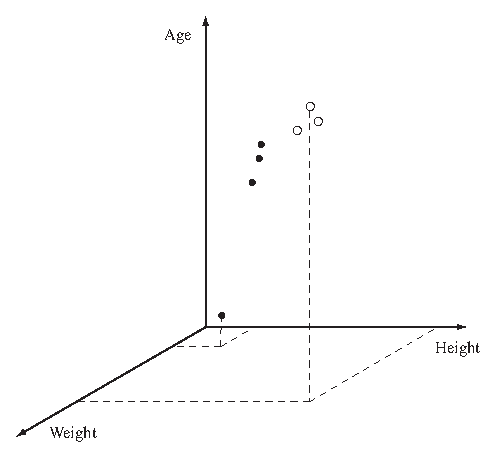
\includegraphics[height=30mm]{figures/fig03-01.eps}

\es

\bs{Linear Algebra}
Linear algebra allows us to describe structures in $n$-dimensional spaces
very effectively.

The representation of the models in support vector machines draw heavily on
concepts such as vector spaces, planes, and norms from linear algebra.

We start with the most basic definition:

\definition{
A directed line segment is called a \ul{vector}.  A vector has
both a length and a direction.  The length is sometimes called the
Euclidean norm or magnitude. A vector of length $1$ is called a 
\ul{unit vector}.
}

A special case of vector is the position vector:

\definition{A \ul{position vector} is a vector whose initial point is the origin
of some coordinate system and whose terminal point is described by a set of
coordinates in the coordinate system.}


\es

\bs{Position Vectors}

Our data set revisited:

\begin{center}
{\tiny
   \begin{tabular}{ l rrr c}
      \toprule
         & Height  & Weight & Age & Gender\\
      \midrule
      Jane      & 25.4 & 32.7 & 2.5 & F \\
      Amanda & 65.2 & 132.0 & 36.5 & F \\
      Paul      & 71.7 & 175.1 & 25.5 & M \\
      Mary      & 62.6 & 126.0 & 31.0 & F \\
      Gary      & 68.2 & 182.0 & 42.5 & M \\
     Betty      & 58.5 & 118.5 & 21.0 & F \\
     John  & 72.0 & 195.2 & 45.2 & M\\
      \bottomrule
   \end{tabular}
}
\end{center}

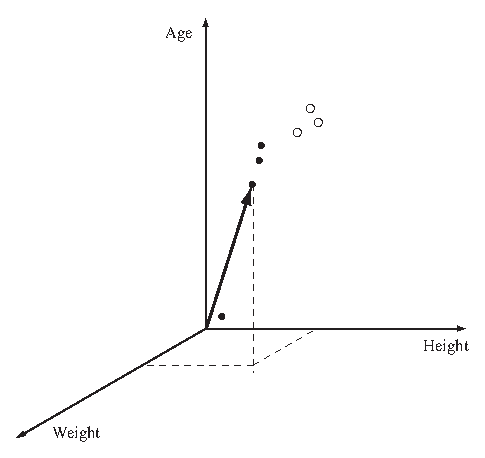
\includegraphics[height=30mm]{figures/fig03-02.eps}

{\bf Example:} The position vector for Betty starts at $(0,0,0)$ and ends at $(58.5,118.5,21.0)$
\es

\bs{Vector Operations}
Vector operations such as {\em equality}, {\em addition}, and {\em scalar multiplication}
are {\em componentwise}.

\example{Let $\ol{a} = (a_1,a_2,a_3)$ and $\ol{b} = (b_1, b_2, b_3)$ be position vectors, then
\[
\ol{a} = \ol{b} \mbox{ iff } a_1 = b_1, a_2 = b_2, a_3 = b_3.
\]}

This gives rise to identities such as
\[
\begin{array}{rclr}
\ol{a} + \ol{b} & = & \ol{b} + \ol{a} & \mbox{(commutativity)}\\
(\ol{a} + \ol{b}) + \ol{c} & = & \ol{a} + (\ol{b} + \ol{c}) & \mbox{(associativity)}\\
\ol{a} + \ol{0} & = & \ol{0} + \ol{a} = \ol{a}& \mbox{(identity)}\\
\ol{a} + (-\ol{a}) & = & \ol{0} & \mbox{ (reciprocal)}
\end{array}
\]
Where  $\ol{a}$,$\ol{b}$, and $\ol{c}$ are position vectors.
Furthermore, $\ol{0} = (0,0,\ldots,0)= 0^n$ is the \ul{null vector} and $(-\ol{a})$ is the 
vector $(-a_1,-a_2,\ldots,-a_n) = -1 \times \ol{a}$.
\es

\bs{More Identities}
\[
\begin{array}{rclr}
q(\ol{a} + \ol{b}) & = & q\ol{a} + q\ol{b} & \mbox{(distributivity)}\\
(p+q)\ol{a} & = & p\ol{a} + q\ol{a} & \mbox{(distributivity)}\\
p(q\ol{a}) & = & (pq)\ol{a} & \mbox{(associativity)}\\
1\ol{a} & = &  \ol{a}& \mbox{(identity)}\\
0\ol{a} & = &  \ol{0}& \\
q\ol{0} & = &  \ol{0}& \\
(-1)\ol{a} & = & -\ol{a} & 
\end{array}
\]
\es

\bs{Vector Spaces}
Informally we say that a vector space is a collection of vector sthat can be added and
scaled.  More formally,

\definition{
A non-empty set $V$ of vectors in $\Rnspace{n}$ is called a 
\ul{(real) vector space} if vector addition and scalar multiplication are defined
and closed
over this set and satisfy the following axioms for all $\ol{a}$, $\ol{b}$, $\ol{c} 
\in V$ and $p,q \in \Real$.\\
Addition:
\[
\begin{array}{rcl}
\ol{a} + \ol{b} & = & \ol{b} + \ol{a} \\
(\ol{a} + \ol{b}) + \ol{c} & = & \ol{a} + (\ol{b} + \ol{c}) \\
\ol{a} + \ol{0} & =  &\ol{a}\\
\ol{a} + (-\ol{a}) & = & \ol{0} 
\end{array}
\]
Multiplication:
\[
\begin{array}{rcl}
q(\ol{a} + \ol{b}) & = & q\ol{a} + q\ol{b}\\
(p+q)\ol{a} & = & p\ol{a} + q\ol{a} \\
p(q\ol{a}) & = & (pq)\ol{a} \\
1\ol{a} & = &  \ol{a}
\end{array}
\]
}

\es

\bs{Linear Combinations}
We can use addition and multiplication in a vector space to construct new
vectors from given ones.

\example{Let $\ol{a}_1$, $\ol{a}_2$, \ldots,$\ol{a}_m$ be vectors in some vector space $V$,
then an expression of the form
\[
\sum_{i = 1}^{m} q_i \ol{a}_i = q_1 \ol{a}_1 + \ldots + q_m \ol{a}_m ,
\]
where $q_i \in \Real$, is called a \ul{linear combination} and 
the closure property of vector spaces guarantees that $\sum_{i = 1}^{m} q_i \ol{a}_i \in V$.
}
\es

\bs{Linear Combinations}
An important example of linear combinations is the formal notion of dimensionality of a data set.

\example{Let the unit vectors $\ol{\imath} = (1,0,0)$, $\ol{\jmath} = (0,1,0)$, and $\ol{k} = (0,0,1)$
be {\em linearly independent} vectors, then we can view them as the {\em canonical basis}
of $\Rnspace{3}$, that is, any vector in $\Rnspace{3}$ can be represented as a linear
combination of these three vectors.}

\example{Consider the position vector for Amanda.
We can rewrite it as,
\begin{equation*}
(65.2,132.0, 36.5) = 65.2(1,0,0) + 132.0(0,1,0) + 36.5(0,0,1).
\end{equation*}
}

{\bf Observation:} The real space $\Rnspace{n}$ can always be considered a vector space.

\es

\bs{The Dot Product}
\definition{
Given two vectors $\ol{a} = (a_1,\ldots,a_n)$ and $\ol{b} = (b_1,\ldots,b_n)$ in
an $n$-dimensional vector space $V$, then we define the \ul{dot product} as the
operation
\begin{equation}
\ol{a}\bullet\ol{b} = a_1 b_1 + \ldots + a_n b_n
\end{equation}
or
\begin{equation}
\ol{a}\bullet\ol{b} = \abs{\ol{a}} \abs{\ol{b}} \cos\gamma,
\end{equation}
where $\abs{\ol{a}} = \sqrt{a_1^2 + \ldots + a_n^2}$ is the length of vector
$\ol{a}$ and $\gamma$ is the angle between the two position vectors.
}

The following identities hold for dot products.  
Let $\ol{a}$, $\ol{b}$, $\ol{c} \in V$ and $p$, $q \in \Real$, then
\[
\begin{array}{rclr}
(p\ol{a} + q\ol{b})\bullet\ol{c} & = & p\ol{a}\bullet\ol{c} + q\ol{b}\bullet\ol{c} & \mbox{(linearity)}\\
\ol{a}\bullet\ol{b} & = & \ol{b}\bullet\ol{a} & \mbox{(symmetry)}\\
\ol{a}\bullet\ol{a} & \ge & 0, \mbox{ and}& \\
\ol{a}\bullet\ol{a} & = & 0 \mbox{ iff } \ol{a} = \ol{0} & \mbox{(positive-definiteness)}
\end{array}
\]
\es

\bs{The Dot Product}

We also have the following interesting identities that are not as fundamental as the
previous set but very useful:
\begin{align*}
\abs{\ol{a}} & =  \sqrt{\ol{a} \bullet \ol{a}},\\
\cos\gamma & =  \frac{\ol{a} \bullet \ol{a}}{\abs{\ol{a}} \abs{\ol{b}}}.
\end{align*}

So what does this mean?  What is the intuition behind the dot product?

\begin{center}
\fbox{The dot product is a {\bf\em measure of similarity}.}
\end{center}

Consider the second equation above with $k = \abs{\ol{a}} \abs{\ol{b}}$, then $\ol{a}\bullet\ol{b} = k \cos\gamma$ and
we see that the value of the dot product is proportional to the cosine of the angle between them: $0^\circ\mapsto k$, $90^\circ\mapsto 0$, $180^\circ\mapsto -k$, {\em etc.}
\begin{center}
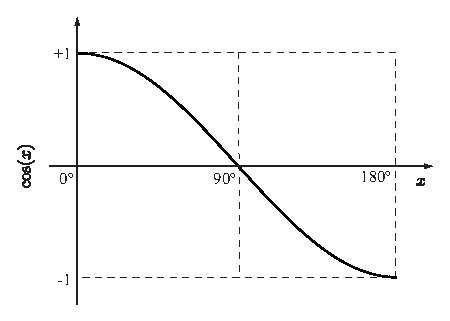
\includegraphics[height=20mm]{figures/fig03-06.eps}
\end{center}
\es

\bs{Dot Product Spaces}
\vspace{.2in}
\definition{A \ul{dot product space} is a vector space where dot products are defined.}

\vspace{.2in}
That is, given any two vectors in the vector space we can measure their similarity.

\vspace{.2in}
\definition{Two non-zero length vectors are \ul{orthogonal} if and only if their dot product is zero (maximum dissimilarity).}

\vspace{.2in}
{\bf Observation:} The real space $\Rnspace{n}$ can always be considered a dot product space.


\es

\bs{Lines \& Dot Products}
We can represent functions using dot products, all of the following identities
describe the same set of points:
\begin{eqnarray*}
f(x) &=& -mx\\
y &=& -mx\\
mx + y &=& 0\\
w_1 x + w_2 y &=& 0, \mbox{ where } w_1 = m, w_2 = 1\\
\ol{w}\bullet\ol{x} &=& 0, \mbox{ where $\ol{w} = (w_1, w_2)$ and $\ol{x} = (x,y)$}
\end{eqnarray*}

{\bf Note:} an advantage of the dot product notation of the last identity
 is that dimensionality is implicit 
rather than explicit as in the other identities allowing us to describe planes and
hyperplanes with very compact notation.

{\bf Note:} the vectors $\ol{w}$ and $\ol{x}$ are orthogonal, and since $\ol{x}$ describes
a line (hyperplane) we call $\ol{w}$ the {\bf\em normal vector} of the line (hyperplane).
\es
\bs{Lines \& Dot Products}
\begin{center}
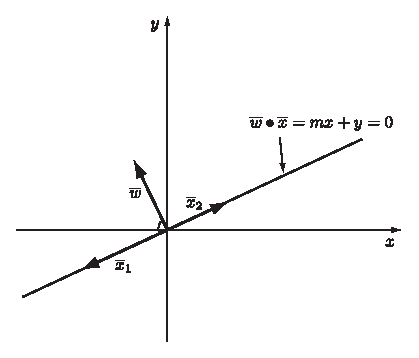
\includegraphics[height=70mm]{figures/fig03-07.eps}
\end{center}
\es

\bs{Lines \& Dot Products}
We can generalize the above expression a little bit by admitting lines that do not
have to go through the origin of the coordinate system:

\[
\ol{w}\bullet\ol{x} = b
\]

 where $\ol{w} = (w_1, w_2)$ and $\ol{x} = (x,y)$.  
 
 The constant $\frac{b}{w_2}$ is called the the {\bf\em $y$-intercept}.
 
 \begin{center}
 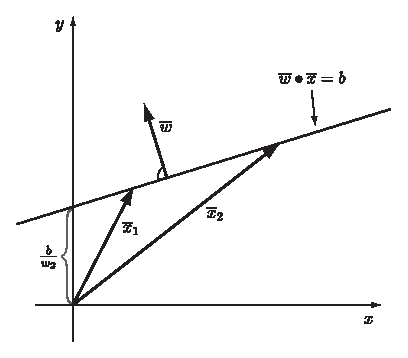
\includegraphics[height=40mm]{figures/fig03-08.eps}
 \end{center}
 \es

\bs{Hyperplanes}
We can generalize this even further by admitting arbitrary dimensions $n > 2$ such that
$\ol{w} = (w_1,\ldots,w_n)$ and
$\ol{x} = (x_1,\ldots,x_n)$.

The dot product notation itself does not change
\begin{center}
\fbox{$\ol{w}\bullet\ol{x} = b$}
\end{center}

This equation defines a {\bf\em hyperplane} in $n$-dimensional space.

\es

\bs{Hyperplanes}
It is difficult to draw hyperplanes, for $n = 3$ hyperplanes degenerate into the well
known $3$-dimensional plane.  

\example{Let $\ol{w} = (w_1, w_2,w_3)$ and $\ol{x} = (x,y,z)$, then
\begin{center}
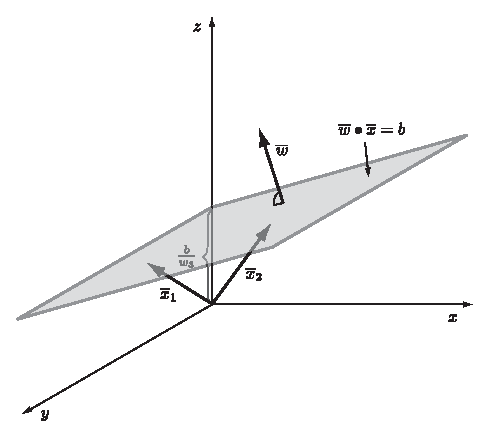
\includegraphics[height=55mm]{figures/fig03-09.eps}
\end{center}
}
\es

\end{document}
%%%%%%%%%%%%%%%%%%%%%%%%%%% end of template1.tex %%%%%%%%%%%%%%%%%%%%%%%%%%%%%%%%

